\documentclass[%
	final, %
	% draft, % Grafische Elemente durch graue Boxen ersetzen (beschleunigt Kompilieren)
	% 8pt, % Zu klein, erfordert Paket extsize
	% 9pt, % Zu klein, erfordert Paket extsize
	% 10pt, % für Folien mit sehr viel Text
	9pt, % Standardschriftgröße
	% 12pt, % etwas größer und daher besser zu lesen
	% 14pt, % deutlich größer, erfordert Paket extsize
	% 17pt, % PowerPoint Standardschriftgröße, erfordert Paket extsize
	% 20pt, % sehr groß, erfordert Paket extsize
	% trans,% Zum Erstellen von Overhead Folien
	% handout, % Erstellen eines Handouts
	% article,% Erstellen eines Artikels
 	% compress, % Die Navigation in der Kopfzeile wird komprimiert dargestellt
	t, % Place text of slides at the (vertical) top of the slides
	% c, % Place text of slides at the (vertical) center of the slides
	% color={}, % list of options for color
	xcolor={table,dvipsnames}, % Optionen für xcolor übergeben
	% hyperref={}, % list of options for hyperref
	% envcountsect, % Causes theorems, definitions, and so on to be numbered locally to each section.
	% notheorems, % Switches off the definition of default blocks like theorem
	% noamsthm, % Does not load amsthm and also not amsmath
	% ucs, % lädt ucs Paket
	% utf8, % lädt utf8x Paket von ucs (utf8 enconding)
	% dvips, % erzwingt das Laden des dvips Treibers - idR nicht nötig!
	% usepdftitle=false, % Suppresses the automatic generation of title and author entries in the pdf document information.
	% ignorenonframetext, % suppresses content created for the article mode ??
	show notes, % enables Notes
	% leqno,
	% fleqn,
]{beamer}[2007/03/11] % Minimum necessary version due to severe bugs in version 3.06 !!!

% ~~~~~~~~~~~~~~~~~~~~~~~~~~~~~~~~~~~~~~~~~~~~~~~~~~~~~~~~~~~~~~~~~~~~~~~~
% Fonts Fonts Fonts
% ~~~~~~~~~~~~~~~~~~~~~~~~~~~~~~~~~~~~~~~~~~~~~~~~~~~~~~~~~~~~~~~~~~~~~~~~
\usepackage[T1]{fontenc} % T1 Schrift Encoding
\usepackage{textcomp}	 % additional symbols (Text Companion font extension)
 
 
% \usepackage{lmodern}               %% --- Latin Modern
\usepackage{mathptmx}              %% --- Times mit Matheschriften
% \usepackage{mathpazo}              %% --- Palantino
% \usepackage{charter}               %% --- Charter
% \usepackage{bookman}               %% Bookman (lädt Avant Garde !!)
% \usepackage{newcent}               %% New Century Schoolbook (lädt Avant Garde !!)
 
% \usepackage{bera}
\usepackage[scaled=.90]{helvet}    %% --- Helvetica (Arial)
% \usepackage{cmbright}              %% --- CM-Bright (eigntlich eine Familie)
% \usepackage{tpslifonts}            %% --- (Font for Slides)
% \usepackage{avant}      	          %% --- Avantgard
%
\usepackage{courier}               %% --- Courier
%\usepackage[scaled=0.9]{luximono}  	 %% --- Luxi Mono

% *** Sprache *****************************
\usepackage[utf8]{inputenc}
\usepackage[T1]{fontenc}
\usepackage[ngerman]{babel}

\usepackage[%
   %final,
   %draft % do not include images (faster)
]{graphicx}
\usepackage{subfigure}
 
\usepackage{xcolor}
\definecolor{boxheadcol}{RGB}{59, 91, 134}
\definecolor{boxcol}{gray}{.9}

\definecolor{avedo}{RGB}{59, 91, 134}
\definecolor{darkgray}{RGB}{69,69,69}
\definecolor{lightgray}{gray}{.9}
\definecolor{darkblue}{RGB}{59, 91, 134}
\definecolor{fgcgray}{rgb}{0.4, 0.4, 0.4}
\definecolor{bgctitle}{RGB}{59, 91, 134}
\definecolor{fgctitle}{rgb}{0.99, 0.99, 0.95}
 
\usepackage{tabularx}   % Erweiterte Tabellen Optionen
\usepackage{booktabs}
\usepackage{multicol}

\usepackage{amssymb,amsmath}
\usepackage{listings}
\usepackage{hyperref}
 
\definecolor{dkgreen}{rgb}{0,0.6,0}
\definecolor{gray}{rgb}{0.5,0.5,0.5}
\definecolor{mauve}{rgb}{0.58,0,0.82}

\lstset{ %
  language=Java, % the language of the code
  basicstyle=\tiny, % the size of the fonts that are used for the code
  numbers=left, % where to put the line-numbers
  numberstyle=\tiny\color{gray}, % the style that is used for the line-numbers
  stepnumber=5, % the step between two line-numbers. If it's 1, each line
  numbersep=5pt, % how far the line-numbers are from the code
  firstnumber=1,
  numberfirstline=false,
  backgroundcolor=\color{white}, % choose the background color. You must add \usepackage{color}
  showspaces=false, % show spaces adding particular underscores
  showstringspaces=false, % underline spaces within strings
  showtabs=false, % show tabs within strings adding particular underscores
  tabsize=3, % sets default tabsize to 2 spaces
  captionpos=b, % sets the caption-position to bottom
  breaklines=true, % sets automatic line breaking
  breakatwhitespace=false, % sets if automatic breaks should only happen at whitespace
  title=\lstname, % show the filename of files included with \lstinputlisting;
  keywordstyle=\color{blue}, % keyword style
  commentstyle=\color{dkgreen}, % comment style
  stringstyle=\color{mauve}, % string literal style
  escapeinside={\%*}{*)}, % if you want to add a comment within your code
  morekeywords={*,...}, % if you want to add more keywords to the set
  xleftmargin=2em,
  xrightmargin=2em,
  aboveskip=1em,
  nolol=true
}

\def\thelstlisting{}
\makeatletter
\AtBeginDocument{%
  \renewcommand \thelstlisting
       {}%
}
\makeatother

% *****************************************
% >>> Themes <<<<<<<<<<<<<<<<<<<<<<<<<<<<<<
% *****************************************
 
% \usetheme[<options>]{<name list>} 		Installs the presentation theme named <name>.
% \usecolortheme[<options>]{<name list>} Same as \usetheme, only for color themes.
% \usefonttheme[<options>]{<name>} 		Same as \usetheme, only for font themes.
% \useinnertheme[<options>]{<name>}		Same as \usetheme, only for inner themes.
% \useoutertheme[<options>]{<name>}		Same as \usetheme, only for outer themes.

 \usetheme[%
 	secheader % section im Header
]{Boadilla}

\useinnertheme{rectangles} 

\usecolortheme[%
 	named=avedo,
]{structure}

\setbeamercolor*{titlelike}{fg=white,bg=avedo}
\setbeamercolor*{title in head/foot}{fg=white,bg=avedo}
\setbeamercolor*{date in head/foot}{fg=white,bg=avedo}
\setbeamercolor*{author in head/foot}{fg=white,bg=avedo}
\setbeamercolor*{normal text}{fg=darkgray}

\setbeamercovered{transparent}




% *****************************************
% >>>> Veraendern der Schrifteinstellung definierter Elemente
% *****************************************
 
% Beispiele
% \setbeamerfont{frametitle}{size=\large}
% \setbeamerfont{frametitle}{series=\bfseries}
 
% weitere Befehle
% size= size command sets the size attribute of the beamerfont.
% size*={ size in pt }{ baselineskip }
% shape= (\itshape, \slshape, \scshape, or \upshape)
% series= (command like \bfseries.)
% family= (command like \rmfamily or \sffamily).
% family*={ family name } (For example, the family name for Times happens to be ptm. )
% parent={ parent list } specifies a list of parent fonts.
%
% Example for parent
% \setbeamerfont{parent A}{size=\large}
% \setbeamerfont{parent B}{series=\bfseries}
% \setbeamerfont{child}{parent={parent A, parent B},size=\small}
%
% \usebeamerfont{child}
% This text is small and bold.




% *****************************************
% >>>> 15.3.2    Using Beamer’s Templates
% *****************************************

\makeatletter
\AtBeginPart{%
  \addtocontents{toc}{\protect\beamer@partintoc{\the\c@part}{\beamer@partnameshort}{\the\c@page}}%
}
%% number, shortname, page.
\providecommand\beamer@partintoc[3]{%
  \ifnum\c@tocdepth=-1\relax
    % requesting onlyparts.
    \makebox[6em]{#1.} #2
    \par
  \fi
}
\define@key{beamertoc}{onlyparts}[]{%
  \c@tocdepth=-1\relax
}
\makeatother%


\makeatletter
\setbeamercolor{secsubsec}{fg=white,bg=avedo}
\setbeamertemplate{headline}
{
  \leavevmode%
  \hbox{%
  \begin{beamercolorbox}[wd=\paperwidth,ht=2.5ex,dp=1ex]{secsubsec}%
    \raggedright
    \hspace*{2em}%
    {\sffamily\scriptsize\insertpart\hfill\insertsection}%
    \hspace*{2em}%
  \end{beamercolorbox}%
  }%
}
\makeatother

\makeatletter
\setbeamercolor{frametitle}{fg=avedo,bg=white}
\setbeamertemplate{frametitle}
{\leavevmode
  \hbox{%
  \begin{beamercolorbox}[wd=\paperwidth,ht=3.5ex,dp=0.7ex]{frametitle}%
    \raggedright\hspace*{1.5em}\Large\insertframetitle
  \end{beamercolorbox}
  }%
}
\makeatother

\makeatletter
\setbeamertemplate{footline}
{
  \leavevmode%
  \hbox{%
  \begin{beamercolorbox}[wd=.333333\paperwidth,ht=2.25ex,dp=1ex,center]{author in head/foot}%
    \usebeamerfont{author in head/foot}\insertshortauthor~~\beamer@ifempty{\insertshortinstitute}{}{(\insertshortinstitute)}
  \end{beamercolorbox}%
  \begin{beamercolorbox}[wd=.333333\paperwidth,ht=2.25ex,dp=1ex,center]{title in head/foot}%
    \usebeamerfont{title in head/foot}\insertshorttitle
  \end{beamercolorbox}%
  \begin{beamercolorbox}[wd=.333333\paperwidth,ht=2.25ex,dp=1ex,right]{date in head/foot}%
    \usebeamerfont{date in head/foot}\insertshortdate{}\hspace*{4em}
  \end{beamercolorbox}}%
  \vskip0pt%
}
\makeatother

\makeatletter
\setbeamertemplate{part page}
{
  \begin{centering}
    \vskip3em\par
    \begin{beamercolorbox}[sep=16pt,center]{part title}
      \usebeamerfont{part title}\insertpart\par
    \end{beamercolorbox}
  \end{centering}
}
\makeatother

\renewenvironment{block}[1]{%
  \begin{actionenv}%
      \def\insertblocktitle{#1}%
      \par%
      \mode<presentation>{%
        \setbeamercolor{block title}{fg=white,bg=avedo}
       \setbeamercolor{block body}{fg=darkgray,bg=lightgray}
       \setbeamercolor{itemize item}{fg=avedo}
       \setbeamertemplate{itemize item}[triangle]
       \setbeamercolor{enumerate item}{fg=avedo}
       \setbeamertemplate{enumerate item}[square]
     }%
      \usebeamertemplate{block begin}}
    {\par\usebeamertemplate{block end}\end{actionenv}}

\renewenvironment{exampleblock}[1]{%
  \begin{actionenv}%
      \def\insertblocktitle{#1}%
      \par%
      \mode<presentation>{%
        \setbeamercolor{block title}{fg=white,bg=avedo}
       \setbeamercolor{block body}{fg=darkgray,bg=lightgray}
       \setbeamercolor{itemize item}{fg=avedo}
       \setbeamertemplate{itemize item}[triangle]
       \setbeamercolor{enumerate item}{fg=avedo}
       \setbeamertemplate{enumerate item}[square]
     }%
      \usebeamertemplate{block begin}}
    {\par\usebeamertemplate{block end}\end{actionenv}}

\renewenvironment{alertblock}[1]{%
  \begin{actionenv}%
      \def\insertblocktitle{#1}%
      \par%
      \mode<presentation>{%
        \setbeamercolor{block title}{fg=white,bg=avedo}
       \setbeamercolor{block body}{fg=darkgray,bg=lightgray}
       \setbeamercolor{itemize item}{fg=avedo}
       \setbeamertemplate{itemize item}[triangle]
       \setbeamercolor{enumerate item}{fg=avedo}
       \setbeamertemplate{enumerate item}[square]
     }%
      \usebeamertemplate{block begin}}
    {\par\usebeamertemplate{block end}\end{actionenv}}

\newenvironment{attrDesc}[1]{%
   \vspace{0.3cm}
   \small
   \begin{center}
      \setlength\arrayrulewidth{0.75pt}
      \arrayrulecolor{white}
      \renewcommand{\arraystretch}{1.3}
      \rowcolors{1}{boxcol}{boxcol}
      \begin{tabular}{#1}
         \rowcolor{boxheadcol}
         \rowstyle{\color{white}\bfseries\sffamily}
}{   
      \end{tabular}
   \end{center}
   \vspace{0.3cm}
}

\newcolumntype{+}{>{\global\let\currentrowstyle\relax}}
\newcolumntype{^}{>{\currentrowstyle}}
\newcommand{\rowstyle}[1]{\gdef\currentrowstyle{#1}%
#1\ignorespaces
}

\setbeamertemplate{mini frames}[box] % shows small rectangles as mini frames.
\setbeamertemplate{navigation symbols}{} % suppresses all navigation symbols:
\setbeamersize{text margin left=2em,text margin right=2em}
\setbeamertemplate{sections/subsections in toc}[square] 
\setbeamertemplate{bibliography item}[default]
\setbeamertemplate{itemize items}[triangle]
\setbeamertemplate{enumerate items}[square]

%% Eigene Definitionen ============================
%

\newcommand{\therfore}{\ding{225}\mbox{ }}
\newcommand{\verythinarrow}{\ding{221}\mbox{ }}
\newcommand{\thinarrow}{\ding{222}\mbox{ }}
\newcommand{\newarrow}{\ding{222}\mbox{ }}
\newcommand{\addspace}{\vspace{0.5\baselineskip}}



\begin{document}
 	\title{Android -- Eine Einführung}
\subtitle{Layouts, Views \& Adapter}
\author[A. Wilhelm]{Andreas Wilhelm}
\institute[IfI -- Uni Göttingen]{
   Institut für Informatik\\ Georg-August-Universität Göttingen
}
\titlegraphic{}
%\date{\today}
\date{www.avedo.net}

\begin{frame}[plain]
  \titlepage
\end{frame}

\section[Contents]{}
\begin{frame}
	\frametitle{Contents}
	\tableofcontents[onlyparts]
\end{frame}

\part{Layouts}
\frame{\partpage}
\begin{frame}
	\frametitle{Contents}
	\tableofcontents[]
\end{frame}

\section{Überblick}
\begin{frame}
   \frametitle{Allgemeines}
   \begin{itemize}
      \item Oberflächen für Aktivitäten, Menüs, Dialogen und Widgets
      \item Grundelemente Views und ViewGroups (Layouts \& AdapterViews)
      \item Deklaration im XML-Format
      \item Formatierung eines Elements über Attribute
      \item Alternativ View-Objekte während der Laufzeit im Quellcode 
         erzeugen und ändern
      \item Weitestgehend einheitliche Namensgebung für XML-Attribute 
         und Objekt-Methoden
   \end{itemize}

   \begin{alertblock}{XML-Layouts}
      Deklaration von Layouts in XML verschlankt den Code, 
      ermöglicht Unterstützung verschiedener Oberflächen, Sprachen 
      und Auflösungen und erleichtert den Debugging-Prozess.
   \end{alertblock}
\end{frame}

\begin{frame}
   \frametitle{Deklaration}
   \begin{itemize}
      \item Erstellung von Layouts erinnert an HTML-Code
      \item Jedes layout darf nur ein Wurzelelement enthalten 
         (View, ViewGroup, Layout, Merge)
      \item Darunter beliebig verschachtelte Layout-Hierarchie
      \item Speichern von Layouts unter \emph{/res/layouts}
      \item Zugriff im Quellcode über automatisch generierte Klasse \emph{R}
      \item Zugriff in anderen Layouts über \emph{@[package:]layout/filename}
   \end{itemize}
\end{frame}

\section{ViewGroups}
\begin{frame}
   \frametitle{Allgemeines}
   \begin{itemize}
      \item Struktur-Elemente, die andere Views anordnen
      \item LinearLayout, das FrameLayout oder das RelativeLayout
      \item Weitere ViewGroups ohne Kindelemente (Bsp: AdapterView)
      \item Basis-Attribute ID (optional), sowie Breite und Höhe
   \end{itemize}

   \begin{alertblock}{Android-IDs}
      Eindeutige ID eines Layout-Elements wird über \emph{android:id} 
      in der Form \emph{@+id/name} deklariert. + signalisiert dabei, dass es sich 
      um eine neue ID handelt. Diese ID kann im Quellcode mit \emph{R.id.name} 
      referenziert werden.\\

      Alternativ kann eine ID als Resource deklariert und mit \emph{@id/name} 
      referenziert werden. Die Deklaration einer solchen Resource wird in XML vorgenommen 
      und unter einem beliebigen Dateinamen unter \emph{/res/values} abgelegt.\\

      \lstinputlisting[
         backgroundcolor=\color{boxcol},language=xml,
         caption=Deklaration von IDs,label={lst:id_resource.xml}]{src/xml/id_resource.xml}
   \end{alertblock}
\end{frame}

\begin{frame}
   \frametitle{Bemaßungen}
   \begin{itemize}
      \item Bemaßungen eines ViewGroups mit den Attributen \emph{android:layout\_width} 
			und \emph{android:layout\_height} entweder explizit oder implizit
      \item Explizite Angabe erfolgt dabei als Wert oder als Resource
      \item Implizite über die Schlüsselwörter \emph{fill\_parent}, 
         \emph{match\_parent} oder \emph{wrap\_content}
   \end{itemize}

   Zur Bemaßungen können verschiedene Einheiten (px, dp, sp, pt, in, mm) 
   oder Schlüsselwörter verwenden.\\

	\begin{attrDesc}{+p{3cm}|^p{7cm}}
		Schlüsselwort & Beschreibung\\
		\hline
      \emph{match\_parent} & Weist aktuellem Objekt die Größe des Eltern-Elements zu 
         (löst \emph{fill\_parent} ab)\\
      \emph{fill\_parent} & Weist aktuellen Objekt die Größe des Eltern-Elements zu\\
      \emph{wrap\_content} & Sorgt für Anpassung der Größe, sodass Inhalt umschlossen wird\\
  	\end{attrDesc}

   Alternativ kann man auch eine Resource im Quellcode über die Klasse \emph{R} 
   oder in einer XMl-Datei mit dem Schlüssel \emph{@[package:]dimen/dimension\_name} 
   referenziert.\\

   \lstinputlisting[
      backgroundcolor=\color{boxcol},language=xml,
      caption=Deklaration von Dimensionen,label={lst:dimen.xml}]{src/xml/dimen.xml}
\end{frame}

\section{View}
\begin{frame}
   \frametitle{Allgemeines}
   \begin{itemize}
      \item Allein stehendes Element einer grafischen Oberfläche
      \item Nimmt rechteckige Fläche des Bildschirms ein
      \item Kümmert sich um die Ausgabe und das Verarbeiten von Ereignissen
      \item Textfelder, Buttons und Eingabefelder, wie beispielsweise \emph{TextView}
      \item Deklaration per XML oder im Quellcode
      \item Verwaltung der Basis-Attribute, wie bei ViewGroups
   \end{itemize}
\end{frame}

\section{RequestFocus}
\begin{frame}
   \frametitle{RequestFocus}
   \begin{itemize}
      \item Gibt View bzw. ViewGroup direkt bei Initialisierung den Fokus
      \item XML-Deklaration als leeres Element \emph{\textless{}requestFocus\textgreater}
      \item Zuweisung eines solchen Elements nur einmal pro Datei
   \end{itemize}
\end{frame}

\section{Include}
\begin{frame}
   \frametitle{Include}
   \begin{itemize}
      \item Verbinden bereits existierender Layouts
      \item Element \emph{\textless{}include\textgreater}
      \item Einziges eigenes Attribut Name des einzubinden Layouts
      \item Optional eine ID, sowie Breite und Höhe des Layouts
      \item Werte überschreiben die Werte des Wurzelknotens im eingebundenen Layout
      \item Änderungen an den Bemaßungen mit \emph{android:layout\_width} und 
      	\emph{android:layout\_height} nur für beide Attribute möglich
   \end{itemize}

   \begin{alertblock}{ViewStub}
      Alternativ kann anstatt des \emph{\textless{}include\textgreater}-Elements 
      auch ein \emph{ViewStub} verwendet werden.
   \end{alertblock}
\end{frame}

\section{Merge}
\begin{frame}
   \frametitle{Merge}
   \begin{itemize}
      \item Wurzelelement um Layouts zu verbinden
      \item Sinnvoll wenn Layouts mit \emph{\textless{}include\textgreater} 
         verbunden werden sollen
      \item Flacherer und dadurch einfacherer Aufbau der View-Hierarchie
   \end{itemize}
\end{frame}

\part{View-Klassen}
\frame{\partpage}
\begin{frame}
	\frametitle{Contents}
	\tableofcontents[]
\end{frame}

\section{TextView}
\begin{frame}
   \frametitle{Allgemeines}
   \begin{itemize}
      \item Ausgabe von Text auf dem Bildschirm
      \item Formatierung über Attribute
   \end{itemize}

	\begin{attrDesc}{+p{4cm}|^p{6cm}}
		Attribut & Beschreibung\\
		\hline
		android:text & Der anzuzeigene Text \\
		android:textSize & Schriftgröße [dimension] \\
		android:textColor & Farbe des Textes [color] \\
		android:textStyle & Stil des Texts (bold, italic, bolditalic) [flag] \\
		android:typeface & Schriftart (normal, sans, serif, monospace) in der 
		   der Text angezeigt werden soll [enum] \\
		android:textAllCaps & Flag um Text in Großbuchstaben auszugeben [boolean] \\
		android:shadowColor & Farbe des Text-Schattens [color] \\
		android:shadowRadius & Radius des Textschattens [double] \\
		android:shadowDx & Verschiebung des Schattens in x-Richtung [double] \\
		android:shadowDy & Verschiebung des Schattens in y-Richtung [double] \\
	\end{attrDesc}
\end{frame}

\begin{frame}
   \frametitle{Deklaration im Layout}
	\lstinputlisting[language=xml,caption=TextView,label={lst:textview.xml}]{src/xml/textview.xml}
\end{frame}

\begin{frame}
   \frametitle{Screenshot}
	\begin{figure}[h!]
	  \centering
	  \includegraphics[width=0.7\textwidth]{pictures/textview.ps}
	  \caption{
		  Das TextView
	  }
	  \label{fig:textview}
	\end{figure}
\end{frame}

\section{EditText}
\begin{frame}
   \frametitle{Allgemeines}
   \begin{itemize}
      \item Abgeleitet von der Klasse TextView
      \item Erlaubt Editieren von Text
      \item Formatierungen, wie bei TextView möglich
   \end{itemize}

	\begin{attrDesc}{+p{4cm}|^p{6cm}}
		Attribut & Beschreibung\\
		\hline
		android:hint & Text der angezeigt werden soll, wenn das Eingabefeld leer ist\\
		android:lines & Höhe des Eingabefeldes in Zeilen\\
		android:maxLength & Maximale Länge der EingabeFarbe des Textes\\
		android:password & Erlaubt das verstecken des eingegeben Texts 
		   und deaktiviert die Autovervollständigung [boolean] \\
		android:textColorHint & Farbe des Stanard-Textes [color] \\
	\end{attrDesc}
\end{frame}

\begin{frame}
   \frametitle{Deklaration im Layout}
	\lstinputlisting[language=xml,caption=EditText,label={lst:edittext.xml}]{src/xml/edittext.xml}
\end{frame}

\begin{frame}
   \frametitle{Screenshot}
	\begin{figure}[h!]
	  \centering
	  \includegraphics[width=0.7\textwidth]{pictures/edittext.ps}
	  \caption{
		  Das Eingabefeld
	  }
	  \label{fig:edittext}
	\end{figure}
\end{frame}

\subsection{Button}
\begin{frame}
   \frametitle{Allgemeines}
   \begin{itemize}
      \item Abgeleitet von der Klasse TextView
      \item Erzeugt anklickbare Schaltfläche
      \item Erlaubt direkte Verlinkung mit Callback-Methode
      \item Alternativ Verwendung von \emph{OnClickListener}
   \end{itemize}

	\begin{attrDesc}{+p{4cm}|^p{6cm}}
		Attribut & Beschreibung\\
		\hline
		android:onClick & Definiert eine Methode der Aktivität, die beim 
			klicken auf den Button ausgeführt werden soll\\
	\end{attrDesc}
\end{frame}

\begin{frame}
   \frametitle{Deklaration im Layout}
	\lstinputlisting[language=xml,caption=Button,label={lst:button.xml}]{src/xml/button.xml}
\end{frame}

\begin{frame}
   \frametitle{Implementierung des Callbacks}
	\lstinputlisting[caption=Button OnClickListener,label={lst:onButtonClicked.java}]{src/java/onButtonClicked.java}
\end{frame}

\begin{frame}
   \frametitle{Screenshot}
	\begin{figure}[h!]
	  \centering
	  \includegraphics[width=0.7\textwidth]{pictures/button.ps}
	  \caption{
		  Der Button
	  }
	  \label{fig:button}
	\end{figure}
\end{frame}

\section{CompoundButton}
\begin{frame}
   \frametitle{Allgemeines}
   \begin{itemize}
      \item Abstrakte View Klasse -- Kann nicht direkt verwendet werden
      \item Abgeleitet von der Klasse Button
      \item Kennt zwei Zustände aktiviert (\emph{checked}) und deaktiviert (\emph{unchecked})
      \item Basis-Klasse für z.B. CheckBox, RadioButton, ToggleButton
   \end{itemize}

	\begin{attrDesc}{+p{4cm}|^p{6cm}}
		Attribut & Beschreibung\\
		\hline
		android:button & Legt ein Bild fest, welches auf 
		   der Schaltfläche angezeigt werden soll [drawable]\\
		android:checked & Gibt den initialen Zustand der Schaltfläche an [boolean]\\
	\end{attrDesc}
\end{frame}

\begin{frame}
   \frametitle{Layout Deklaration}
	\lstinputlisting[language=xml,caption=CompoundButton,label={lst:compound_button.xml}]{src/xml/compound_button.xml}
\end{frame}

\section{CheckBox}
\begin{frame}
   \frametitle{Allgemeines}
   \begin{itemize}
      \item Abgeleitet von der Klasse CompoundButton
      \item Kennt zwei Zustände aktiviert (\emph{checked}) und deaktiviert (\emph{unchecked})
   \end{itemize}

	\lstinputlisting[language=xml,caption=CheckBox,label={lst:checkbox.xml}]{src/xml/checkbox.xml}
\end{frame}

\begin{frame}
   \frametitle{Screenshot}
	\begin{figure}[h!]
	  \centering
	  \includegraphics[width=0.7\textwidth]{pictures/checkbox.ps}
	  \caption{
		  Eine Liste von CheckBoxen
	  }
	  \label{fig:checkbox}
	\end{figure}
\end{frame}

\begin{frame}
   \frametitle{Callback Implementierung}
   \begin{itemize}
      \item Verwendung mehrerer zusammengehöriger Checkboxen möglich
      \item Zuweisung eines Callbacks über \emph{android:onClick}-Attribut
      \item Nutzung des gleichen Callbacks möglich
   \end{itemize}

	\lstinputlisting[caption=Methode für mehrere CheckBoxen,label={lst:onGameCbxClicked.java}]{src/java/onGameCbxClicked.java}
\end{frame}

\section{ToggleButton}
\begin{frame}
   \frametitle{Allgemeines}
   \begin{itemize}
      \item Abgeleitet von der Klasse CompoundButton
      \item Kennt zwei Zustände aktiviert (\emph{checked}) und deaktiviert (\emph{unchecked})
      \item Dient als An- und Aus-Schalter 
      \item Weißt jedem Zustand einen Namen zu
   \end{itemize}

	\lstinputlisting[language=xml,caption=ToggleButton,label={lst:toggle_button.xml}]{src/xml/toggle_button.xml}
\end{frame}

\begin{frame}
   \frametitle{Alternative: Slider}
   \begin{itemize}
      \item Eingeführt in Android 4.0
      \item Abgeleitet von der Klasse CompoundButton
      \item Verhalten wie ToggleButton
      \item Ausgabe als Slider
   \end{itemize}

	\lstinputlisting[language=xml,caption=Switch,label={lst:switch.xml}]{src/xml/switch.xml}
\end{frame}

\begin{frame}
   \frametitle{Screenshot}
	\begin{figure}[h!]
	  \centering
	  \includegraphics[width=0.7\textwidth]{pictures/toggle_switches.ps}
	  \caption{
		  ToggleButtons \& Switches
	  }
	  \label{fig:toggle_switches}
	\end{figure}
\end{frame}

\section{RadioButton}
\begin{frame}
   \frametitle{Allgemeines}
   \begin{itemize}
      \item Abgeleitet von der Klasse CompoundButton
      \item Einmal aktiviert immer aktiviert
      \item Gruppierung in RadioGroup sinnvoll
   \end{itemize}

	\lstinputlisting[language=xml,caption=RadioButton,label={lst:radio_button.xml}]{src/xml/radio_button.xml}
\end{frame}

\begin{frame}
   \frametitle{Screenshot}
	\begin{figure}[h!]
	  \centering
	  \includegraphics[width=0.7\textwidth]{pictures/radio_button.ps}
	  \caption{
		  RadioButton
	  }
	  \label{fig:radio_button}
	\end{figure}
\end{frame}

\section{RadioGroup}
\begin{frame}
   \frametitle{Allgemeines}
   \begin{itemize}
      \item Abgeleitet von der Klasse LinearLayout
      \item Dienen der Gruppierung von RadioButtons
      \item Immer nur ein einzelner RadioButton aktiviert
   \end{itemize}
\end{frame}

\begin{frame}
   \frametitle{Deklaration im Layout}
	\lstinputlisting[language=xml,caption=RadioGroup,label={lst:radio_group.xml}]{src/xml/radio_group.xml}
\end{frame}

\begin{frame}
   \frametitle{Screenshot}
	\begin{figure}[h!]
	  \centering
	  \includegraphics[width=0.7\textwidth]{pictures/radio_group.ps}
	  \caption{
		  RadioButtons in einer RadioGroup
	  }
	  \label{fig:radio_group}
	\end{figure}
\end{frame}

\section{CheckedTextView}
\begin{frame}
   \frametitle{Allgemeines}
   \begin{itemize}
      \item Abgeleitet von TextView
      \item Implementiert das Checkable Interface
      \item Kennt Zustände aktiviert (\emph{checked}) und deaktiviert (\emph{unchecked})
      \item Einsatz sinnvoll mit Spinnern und ListViews, wenn \emph{setChoiceMode()} 
      	auf \emph{CHOICE\_MODE\_NONE} gesetzt
   \end{itemize}
\end{frame}

\begin{frame}
   \frametitle{Deklaration im Layout}
	\lstinputlisting[language=xml,caption=CheckedTextView,label={lst:checked_textview.xml}]{src/xml/checked_textview.xml}
\end{frame}

\begin{frame}
   \frametitle{Screenshot}
	\begin{figure}[h!]
	  \centering
	  \includegraphics[width=0.7\textwidth]{pictures/checked_textview.ps}
	  \caption{
		  CheckedTextView
	  }
	  \label{fig:checked_textview}
	\end{figure}
\end{frame}

\section{ImageView}
\begin{frame}
   \frametitle{Allgemeines}
   \begin{itemize}
      \item Anzeige eines Bildes
      \item Kümmert sich um die Bemaßung des Bildes
      \item Formatierungen (Bsp. Einfärbung) über Attribute möglich
   \end{itemize}

	\begin{attrDesc}{+p{4cm}|^p{6cm}}
		Attribut & Beschreibung\\
		\hline
		android:src & Die zu verwendende Bilddatei [drawable]\\
		android:tint & Farbe für Bildeinfärbung [color]\\
		android:adjustViewBounds & Legt fest, ob das ImageView seine Bemaßung an die 
		   seines Bildes anpasst [boolean]\\
		android:scaleType & Legt fest, wie das Bild skaliert und bewegt werden soll 
		   um die erlaubten Bemaßungen einzuhalten [enum]\\
		android:cropToPadding & Legt fest ob ein Bild zugeschnitten werden soll 
		   um in seinen Bereich zu passen [boolean]\\
		android:baselineAlignBottom & Legt fest ob das Bild an der Grundlinie basierend 
		   auf der unteren kante ausgerichtet wird [boolean]\\
		android:baseline & Legt die Grundlinie des Bildes fest [flag]\\ 
		android:maxHeight & Maximale Höhe [dimension]\\
		android:maxWidth & Maximale Breite [dimension]\\
	\end{attrDesc}
\end{frame}

\begin{frame}
   \frametitle{Deklaration im Layout}
	\lstinputlisting[language=xml,caption=ImageView,label={lst:imageview.xml}]{src/xml/imageview.xml}
\end{frame}

\begin{frame}
   \frametitle{Screenshot}
	\begin{figure}[h!]
	  \centering
	  \includegraphics[width=0.7\textwidth]{pictures/imageview.ps}
	  \caption{
		  ImageView
	  }
	  \label{fig:imageview}
	\end{figure}
\end{frame}

\section{ImageButton}
\begin{frame}
   \frametitle{Allgemeines}
   \begin{itemize}
      \item Abgeleitet von ImageView
      \item Sieht normalerweise aus wie Button mit Bild
      \item Angabe von Callback mit \emph{android:onClick}
   \end{itemize}
\end{frame}

\begin{frame}
   \frametitle{Deklaration im Layout}
	\lstinputlisting[language=xml,caption=ImageButton,label={lst:imagebutton.xml}]{src/xml/imagebutton.xml}
\end{frame}

\begin{frame}
   \frametitle{Implementierung des Callbacks}
	\lstinputlisting[caption=Methode onImageButtonClicked,label={lst:onImageButtonClicked.java}]{src/java/onImageButtonClicked.java}
\end{frame}

\begin{frame}
   \frametitle{Screenshot}
	\begin{figure}[h!]
	  \centering
	  \includegraphics[width=0.7\textwidth]{pictures/imagebutton.ps}
	  \caption{
		  ImageButton
	  }
	  \label{fig:imagebutton}
	\end{figure}
\end{frame}

\begin{frame}
   \frametitle{Anmerkung}
	\begin{alertblock}{Event-Hintergründe}
		Es ist möglich die Änderung der Hintergrundfarbe 
		bei verschiedenen Benutzeraktionen, wie beispielsweise einem Klick, selbst 
		festzulegen. Zu diesem Zweck kann man in XML einen \emph{selector} 
		definieren, der anhand der verschiedenen Button-Zustände ein Bild auswählt.

		\vspace{3mm}

		\lstinputlisting[
		   backgroundcolor=\color{boxcol},language=xml,
		   caption=Deklaration von Button-Farben,label={lst:button_drawable.xml}]{src/xml/button_drawable.xml}

		\vspace{3mm}

		Diese Datei legt man wie ein normales Bild unter \emph{/res/drawable} ab.
	\end{alertblock}
\end{frame}

\section{ProgressBar}
\begin{frame}
   \frametitle{Allgemeines}
   \begin{itemize}
      \item Visualisierung des Fortschritts eines laufenden Prozesses
      \item Unterscheidung in nicht deterministisch und deterministisch
      \item Möglichkeit einen zweiten Ladebalken anzuzeigen (Bsp. Buffering)
   \end{itemize}
   
   Android bietet verschiedene Styles, die über das Attribut \emph{style} 
   in der Form \emph{@android:style/style\_name} ausgewählt werden:

	\begin{itemize}
		\item Widget.ProgressBar.Inverse
		\item Widget.ProgressBar.Horizontal
		\item Widget.ProgressBar.Small
		\item Widget.ProgressBar.Small.Inverse
		\item Widget.ProgressBar.Large
		\item Widget.ProgressBar.Large.Inverse
	\end{itemize}
\end{frame}

\begin{frame}
   \frametitle{Attribute}
	\begin{attrDesc}{+p{4cm}|^p{6cm}}
		Attribut & Beschreibung\\
		\hline
		android:indeterminate & Aktiviert den \emph{indeterminate} Modus einer ProgressBar \\
		android:max & Legt den maximalen Wert fest [double]\\
		android:maxHeight & Maximale Höhe der Bar [dimension]\\
		android:maxWidth & Maximale Breite der Bar [dimension]\\
		android:minHeight & Minimale Höhe der Bar [dimension]\\
		android:minWidth & Minimale Breite der Bar [dimension]\\
		android:progress & Der Wert des aktuellen Fortschritts (zwischen 0 und max) \\
		android:progressDrawable & Bild die ProgressBar\\
		android:secondaryProgress & Der Wert des aktuellen sekundären Fortschritts (zwischen 0 und max) \\
	\end{attrDesc}
\end{frame}

\begin{frame}
   \frametitle{Deklaration im Layout}
	\lstinputlisting[language=xml,caption=ProgressBar,label={lst:progressbar.xml}]{src/xml/progressbar.xml}
\end{frame}

\begin{frame}
   \frametitle{Screenshot}
   \begin{figure}[h!]
	  \centering
	  \includegraphics[width=0.7\textwidth]{pictures/progressbar.ps}
	  \caption{
		  ProgressBar
	  }
	  \label{fig:progressbar}
	\end{figure}
\end{frame}

\begin{frame}
   \frametitle{Implementierung}
	\lstinputlisting[caption=Aktualisierung einer ProgressBar,label={lst:progressbar.java}]{src/java/progressbar.java}
\end{frame}

\section{Spinner}
\begin{frame}
   \frametitle{Allgemeines}
   \begin{itemize}
      \item Stellen ein DropDown-Menü bereit
      \item Alternativ anzeige als Dialog
      \item Platz sparende Alternative zu RadioGroups
      \item Initialisierung mit einem Start-Wert möglich
   \end{itemize}
   
   \begin{attrDesc}{+p{4cm}|^p{6cm}}
		Attribut & Beschreibung\\
		\hline
		android:dropDownWidth & Breite des DropDowns für Spinner im DropDown-Modus\\
		android:popupBackground & Hintergrundbild für Spinner im DropDown-Modus\\
		android:prompt & Titel des Spinner Dialogs [resource]\\
		android:spinnerMode & Anzeige Modus eines Spinners (dialog, dropdown) [int]\\
	\end{attrDesc}
\end{frame}

\begin{frame}
   \frametitle{Deklaration im Layout}
	\lstinputlisting[language=xml,caption=Spinner,label={lst:spinner.xml}]{src/xml/spinner.xml}
\end{frame}

\begin{frame}
   \frametitle{Implementierung}
	\lstinputlisting[caption=Ein Spinner-Adapter,label={lst:spinner.java}]{src/java/spinner.java}
\end{frame}

\begin{frame}
   \frametitle{Screenshot}
	\begin{figure}[h!]
	  \centering
	  \includegraphics[width=0.7\textwidth]{pictures/spinner.ps}
	  \caption{
		  Spinner
	  }
	  \label{fig:spinner}
	\end{figure}
\end{frame}


\begin{frame}
   \frametitle{Anmerkung}
	\begin{alertblock}
		Auswahllisten, wie Spinner, können mit String-Array-Resourcen befüllt und 
		sprachunabhängig gestaltet werden. Deklaration in der Sprachdatei 
		\emph{string.xml} unter \emph{/res/values}. 

		\vspace{3mm}

		\lstinputlisting[
		   backgroundcolor=\color{boxcol},language=xml,
		   caption=Deklaration eines String-Arrays,label={lst:string_array.xml}]{src/xml/string_array.xml}
	\end{alertblock}
\end{frame}

\section{Chronometer}
\begin{frame}[label=chronometer]
   \frametitle{Allgemeines}
   \begin{itemize}
      \item Benutzeroberfläche für Timer
      \item Abgeleitet von Klasse \emph{TextView}
      \item Startwert mit \emph{elapsedRealtime()} Mathode aus 
         \emph{SystemClock} Klasse setzen
      \item Alternativ: Automatisch mit \emph{start()} initialisieren
      \item Format \emph{MM:SS} oder \emph{H:MM:SS}
      \item Format kann mit \emph{setFormat(String)} geändert werden
   \end{itemize}

   \begin{attrDesc}{+p{4cm}|^p{6cm}}
      Attribut & Beschreibung\\
      \hline
      android:format & String der ein Ausgabeformat festlegt. Das erste Vorkommen 
         von \emph{\%s} wird durch den aktuellen wert des Timers im Format 
         \emph{MM:SS} oder \emph{H:MM:SS} ersetzt.\\
   \end{attrDesc}
\end{frame}

\begin{frame}
   \frametitle{Deklaration im Layout}
   \lstinputlisting[language=xml,caption=Chronometer,label={lst:chronometer.xml}]{src/xml/chronometer.xml}
\end{frame}

\begin{frame}
   \frametitle{Implementierung}
   \lstinputlisting[caption=Implementierung des Timers,label={lst:chronometer.java}]{src/java/chronometer.java}
\end{frame}

\begin{frame}
   \frametitle{Screenshot}
   \begin{figure}[h!]
     \centering
     \includegraphics[width=0.7\textwidth]{pictures/chronometer.ps}
     \caption{
        Chronometer
     }
     \label{fig:chronometer}
   \end{figure}
\end{frame}

\section{WebView}
\begin{frame}[label=webview]
   \frametitle{Allgemeines}
   \begin{itemize}
      \item Ermöglicht Anzeige von Webseiten innerhalb einer Applikation
      \item Abgeleitet von der Klasse \emph{ViewGroups} oder genauer von \emph{AbsolutLayout}
      \item Anzeigen der Webinhalte übernimmt die \emph{WebKit} Engine
      \item Unterstützt nicht von Haus aus Web typische Besonderheiten, wie JavaScript
      \item Inhalte mit \emph{loadUrl()} oder HTML-Code mit \emph{loadData()} laden
   \end{itemize}

   \begin{alertblock}{Zugriffsrechte für das Internet}
      Um einer Applikation den Zugriff auf das Internet zu ermöglichen, benötigt sie 
      die entsprechenden Rechte. Das bedeutet, dass in der Android Manifest-Datei 
      diese Rechte gesetzt werden müssen. Dazu muss die Zeile aus 
      Listing~\ref{lst:internet_permissions.xml} eingebunden werden.

      \vspace{5mm}

      \lstinputlisting[
         backgroundcolor=\color{boxcol},language=xml,caption=Internet Zugriffsrechte,
         label={lst:internet_permissions.xml}]{src/xml/internet_permissions.xml} 
   \end{alertblock}
\end{frame}

\begin{frame}
   \frametitle{Web 2.0 Funktionen}
   \begin{alertblock}{JavaScript einschalten}
      Auch wenn ein WebView nicht standardmäßig JavaScript unterstützt kann diese 
      Funktionalität aktiviert werden. Zu diesem Zweck verwaltet jedes WebView 
      seine Einstellungen in einem \emph{WebSettings} Objekt, auf das mit der 
      Methode \emph{getSettings()} zugegriffen werden kann. Mit einem Aufruf 
      der Methode \emph{setJavaScriptEnabled(true)} der Klasse WebSettings 
      kann die Unterstützung von JavaScript für das entsprechende WebView aktiviert werden.
   \end{alertblock}

   \begin{alertblock}{HTML-Standard}
      Man muss bei der Verwendung von WebView immer darauf achten, dass es nicht 
      nur Probleme mit komplexeren Webseiten hat, die JavaScript oder Flash einbinden, 
      sondern dass es auch Einschränkungen in Bezug auf den HTML-Code macht.
   \end{alertblock}
\end{frame}

\begin{frame}
   \frametitle{Funktionalitäten erweitern}
   \begin{description}
      \item[WebChromeClient] Kümmert sich um die Verarbeitung von Events, die die 
         grafische Oberfläche beeinflussen.
      \item[WebViewClient]  Kümmert sich um die Verarbeitung von Events, die die 
         Anzeige des Inhalts beeinflussen.
      \item[WebSettings] Änderungen an den Einstellungen, wie Aktivierung von JavaScript.
   \end{description}

   \begin{alertblock}{Web-Applikationen}
      Mit WebView ist es möglich bereits existierende Web-Applikationen direkt 
      in Android zu integrieren.

      \vspace{5mm}

      Dazu wird es ermöglicht Teile des oftmals in Web-Applikationen verwendeten 
      JavaScript-Codes an Android-Code zu binden. So ist es beispielsweise möglich 
      alle Ausgaben, die durch ein JavaScript-Alert erzeugt würden in Android-Toasts 
      ausgeben zu lassen. Android ermöglicht dies durch die Implementierung 
      von \emph{JavaScriptInterfaces}.
   \end{alertblock}
\end{frame}

\section{TimePicker}
\begin{frame}[label=timepicker]
   \frametitle{Allgemeines}
   \begin{itemize}
      \item \emph{TimePicker} ist abgeleitet von Klasse \emph{FrameLayout}
      \item Oberfläche zur Auswahl einer Uhrzeit im AM/PM-Format
   \end{itemize}

   \lstinputlisting[language=xml,caption=TimePicker,label={lst:timepicker.xml}]{src/xml/timepicker.xml}
\end{frame}

\begin{frame}
   \frametitle{Screenshot}
   \begin{figure}[h!]
     \centering
     \includegraphics[width=0.7\textwidth]{pictures/timepicker.ps}
     \caption{
        TimePicker
     }
     \label{fig:timepicker}
   \end{figure}
\end{frame}

\section{DatePicker}
\begin{frame}[label=datepicker]
   \frametitle{Allgemeines}
   \begin{itemize}
      \item \emph{DatePicker} ist abgeleitet von Klasse \emph{FrameLayout}
      \item Oberfläche zur Auswahl eines Datums
      \item Kann als mehrerer Spinner oder Kalender (\emph{CalendarView}) angezeigt werden
   \end{itemize}

   \begin{attrDesc}{+p{4cm}|^p{6cm}}
      Attribut & Beschreibung\\
      \hline
      android:startYear & Das erste Jahr, das als Eingabe möglich sein soll [int]\\
      android:endYear & Das letzte Jahr, das als Eingabe möglich sein soll [int]\\
      android:maxDate & Das minimal angezeigte Datum im CalendarView (Format: mm/dd/yyyy) [string]\\
      android:minDate & Das maximal angezeigte Datum im CalendarView (Format: mm/dd/yyyy) [string]\\
      android:spinnersShown & Gibt an ob Spinner angezeigt werden sollen [boolean]\\
      android:calendarViewShown & Gibt an ob ein CalendarView angezeigt werden soll [boolean]\\
   \end{attrDesc}
\end{frame}

\begin{frame}
   \frametitle{Deklaration im Layout}
   \lstinputlisting[language=xml,caption=DatePicker,label={lst:datepicker.xml}]{src/xml/datepicker.xml}
\end{frame}

\begin{frame}
   \frametitle{Screenshot}
   \begin{figure}[h!]
     \centering
     \includegraphics[width=0.7\textwidth]{pictures/datepicker.ps}
     \caption{
        DatePicker
     }
     \label{fig:datepicker}
   \end{figure}
\end{frame}

\part{ViewGroup-Klassen}
\frame{\partpage}
\begin{frame}
	\frametitle{Contents}
	\tableofcontents[]
\end{frame}

\section{LinearLayout}
\begin{frame}[label=linearlayout]
   \frametitle{Allgemeines}
   \begin{itemize}
      \item Ermöglicht eine horizontale oder vertikale Anordnung seiner Kindelemente
      \item Reihenfolge in der Definition der Kindelemente wird eingehalten
      \item Kann als mehrerer Spinner oder Kalender (\emph{CalendarView}) angezeigt werden
      \item Unterstützt Gewichtungen von Kindelementen (\emph{android:layout\_weight})
   \end{itemize}

   \begin{attrDesc}{+p{4cm}|^p{6cm}}
      Attribut & Beschreibung\\
      \hline
      android:divider & Definiert ein Drawable, das als Trenner zwischen vertikal 
         angeordneten Elementen angezeigt wird [drawable]\\
      android:gravity & Definiert, wie der Inhalt des Layouts angeordnet werden 
         soll [int]\\
      android:measureWithLargestChild & Falls dieses Flag aktiviert wird, 
         werden alle Kindelemente mit gewichtung dazu gezwungen ihre minimale 
         Größe an die des größten Elements anzupassen[boolean]\\
      android:orientation & Legt fest, ob die Kindelemente horizontal oder vertikal angeordnet werden [int]\\
      android:weightSum & Legt die maximale Summe der Gewichtungen fest\\
   \end{attrDesc}
\end{frame}

\begin{frame}
   \frametitle{Gewichtung}
   \begin{alertblock}{Layouts gewichten}
      Um allen Kindelementen eines LinearLayouts den gleichen Raum zu geben 
      kann die Breite des Kindelements im horizontalen Layout auf \emph{0dp}, 
      im vertikalen Layout die Höhe auf \emph{0dp} gesetzt werden. Damit dies 
      jedoch funktioniert müssen alle Kindelement mit 1 gewichtet werden. Dazu 
      setzt man das Attribut \emph{android:layout\_weight} jedes Kindelemnts auf 1.
   \end{alertblock}
\end{frame}

\begin{frame}
   \frametitle{Layout}
   \lstinputlisting[language=xml,caption=LinearLayout,label={lst:linear_layout.xml}]{src/xml/linear_layout.xml}
\end{frame}

\begin{frame}
   \frametitle{Screenshot}
   \begin{figure}[h!]
     \centering
     \includegraphics[width=0.7\textwidth]{pictures/linear_layout.ps}
     \caption{
        LinearLayout
     }
     \label{fig:linear_layout}
   \end{figure}
\end{frame}

\section{RelativeLayout}
\begin{frame}[label=relativelayout]
   \frametitle{Allgemeines}
   \begin{itemize}
      \item Ordnet seine Kindelemente relativ zueinander an
      \item View kann seine Position relativ zu anderen Views auf der selben 
         Ebene oder zum Vater-Element angeben kann
   \end{itemize}

   \begin{attrDesc}{+p{4cm}|^p{6cm}}
      Attribut & Beschreibung\\
      \hline
      android:gravity & Legt fest, wie der Inhalt innerhalb des Views positioniert werden soll [int]\\
      android:ignoreGravity & Legt fest welches View das \emph{android:gravity} Attribut ignoriert [int]\\
      android:layout\_alignParentTop & Legt die Oberkante des Kindelements an die Oberkante des Vaters [boolean]\\
      android:layout\_centerInParent & Zentriert das Kindelement vertikal und horizontal in seinem Vater[boolean]\\
      android:layout\_centerHorizontal & Zentriert das Kindelement horizontal in seinem Vater[boolean]\\
      android:layout\_centerVertical & Zentriert das Kindelement vertikal in seinem Vater[boolean]\\
      android:layout\_above & Positioniert das Element über dem View dessen ID angegeben wurde [resource]\\
      android:layout\_below & Positioniert das Element unter dem View dessen ID angegeben wurde [resource]\\
      android:layout\_toRightOf & Positioniert das Element rechts neben dem View dessen ID angegeben wurde [resource]\\
      android:layout\_toLeftOf & Positioniert das Element links neben dem View dessen ID angegeben wurde [resource]\\
   \end{attrDesc}
\end{frame}

\begin{frame}
   \frametitle{Deklaration im Layout}
   \lstinputlisting[language=xml,caption=RelativeLayout,label={lst:relative_layout.xml}]{src/xml/relative_layout.xml}
\end{frame}

\begin{frame}
   \frametitle{Screenshot}
   \begin{figure}[h!]
     \centering
     \includegraphics[width=0.7\textwidth]{pictures/relative_layout.ps}
     \caption{
        RelativeLayout
     }
     \label{fig:relative_layout}
   \end{figure}
\end{frame}

\section{FrameLayout}
\begin{frame}[label=framelayout]
   \frametitle{Allgemeines}
   \begin{itemize}
      \item Hält einen gewissen Bereich auf dem Bildschirm für ein einzelnes View frei
      \item Mehrere Kindelemente in einem FrameLayout können sich überlappen
      \item Größe des FrameLayouts wird durch größtes Kindelement festgelegt (zzgl. Padding) 
      \item Egal ob Kinder sichtbar oder nicht
   \end{itemize}

   \begin{attrDesc}{+p{4cm}|^p{6cm}}
      Attribut & Beschreibung\\
      \hline
      android:foreground & Legt ein Bild fest, dass über dem Inhalt gezeichnet werden soll [drawable]\\
      android:foregroundGravity & Legt die Ausrichtung des Bildes fest [int]\\
      android:measureAllChildren & Legt fest ob die Bemaßung aller Kindelemente angepasst werden soll [boolean]\\
   \end{attrDesc}
\end{frame}

\begin{frame}
   \frametitle{Deklaration im Layout}
   \lstinputlisting[language=xml,caption=FrameLayout,label={lst:frame_layout.xml}]{src/xml/frame_layout.xml}
\end{frame}

\begin{frame}
   \frametitle{Screenshot}
   \begin{figure}[h!]
     \centering
     \includegraphics[width=0.7\textwidth]{pictures/frame_layout.ps}
     \caption{
        FrameLayout
     }
     \label{fig:frame_layout}
   \end{figure}
\end{frame}

\section{TableLayout}
\begin{frame}[label=tablelayout]
   \frametitle{Allgemeines}
   \begin{itemize}
      \item Platziert Inhalte in einer Tabellenstruktur
      \item Zeilen werden explizit angegeben, Spalten implizit angenommen werden
      \item Größe des FrameLayouts wird durch größtes Kindelement festgelegt (zzgl. Padding) 
      \item Egal ob Kinder sichtbar oder nicht
   \end{itemize}

   \begin{attrDesc}{+p{4cm}|^p{6cm}}
      Attribut & Beschreibung\\
      \hline
      android:collapseColumns & Index der Spalten die zusammengefügt werden sollen (beginnend bei Null) [int,boolean]\\
      android:shrinkColumns & Spalten werden automatisch verkleinert [boolean]\\
      android:stretchColumns & Spalten werden automatisch vergrößert [boolean]\\
      android:layout\_column & Spalte in der ein View eingefügt werden soll [int]\\
      android:layout\_span & Anzahl an Spalten die ein View einnehmen soll [int]\\
   \end{attrDesc}
\end{frame}

\begin{frame}
   \frametitle{Deklaration im Layout}
   \lstinputlisting[language=xml,caption=TableLayout,label={lst:table_layout.xml}]{src/xml/table_layout.xml}
\end{frame}

\begin{frame}
   \frametitle{Screenshot}
   \begin{figure}[h!]
     \centering
     \includegraphics[width=0.7\textwidth]{pictures/table_layout.ps}
     \caption{
        TableLayout
     }
     \label{fig:table_layout}
   \end{figure}
\end{frame}

\section{ScrollView}
\begin{frame}[label=scrollview]
   \frametitle{Allgemeines}
   \begin{itemize}
      \item ScrollView von FrameLayout abgeleitet
      \item Erlaubt, dass das Layout größer ist als das eigentliche Display erlaubt
      \item Kann nur ein Kind enthalten
      \item Egal ob Kinder sichtbar oder nicht
   \end{itemize}

   \begin{alertblock}{ListViews}
		Auch wenn dies möglich ist, sollte man ein ScrollView niemals mit einem ListView 
		verwenden, da sich dies bereits selbst um das scrollen seiner Elemente kümmert. 
		Sollte man dies dennoch tun, zwingt man das ListView dazu sich auf die benötigte 
		länge auszudehnen um alle Elemente anzeigen zu können. Dies würde dafür sorgen, 
		dass die in ListView implementierten Optimierungen zur Anzeige großer Listen 
		umgangen werden.
   \end{alertblock}
\end{frame}

\begin{frame}
   \frametitle{Attribute}

   \begin{attrDesc}{+p{4cm}|^p{6cm}}
      Attribut & Beschreibung\\
      \hline
      android:fillViewport & Ermöglicht es den Inhalt so auszudehnen, dass er den 
         verfügbaren Display-Bereich nutzt [boolean]\\
   \end{attrDesc}

   \begin{alertblock}{Horizontales Scrollen}
		Ein ScrollView kümmert sich nur um das vertikale Scrollen seines Inhalts. Sollte 
		es einmal nötig sein den Inhalt horizontal zu scrollen, so sollte man auf die 
		Klasse HorizontalScrollView zurückgreifen.
   \end{alertblock}
\end{frame}

\begin{frame}
   \frametitle{Deklaration im Layout}
   \lstinputlisting[language=xml,caption=ScrollView,label={lst:scrollview.xml}]{src/xml/scrollview.xml}
\end{frame}

\begin{frame}
   \frametitle{Screenshot}
   \begin{figure}[h!]
     \centering
     \includegraphics[width=0.7\textwidth]{pictures/scrollview.ps}
     \caption{
        ScrollView
     }
     \label{fig:scrollview}
   \end{figure}
\end{frame}

\part{AdapterView-Klassen}
\frame{\partpage}
\begin{frame}
	\frametitle{Contents}
	\tableofcontents[]
\end{frame}

\section{ListView}
\begin{frame}[label=listview]
   \frametitle{ListView}
   \begin{itemize}
      \item Scrollbare Liste von Einträgen
      \item Nutzt spezielle Aktivität ListActivity
      \item ListActivity nutzt automatisch ein Standard-Layout
      \item Eigenes Layout kann mit \emph{setContentView()} gesetzt werden
      \item Liste muss ID \emph{@android:id/list} tragen
      \item View für leere Listen muss ID \emph{@android:id/empty} tragen
   \end{itemize}

   \begin{alertblock}{ListViews \& ScrollView}
		Auch wenn dies möglich ist, sollte man ein ScrollView niemals mit einem ListView 
		verwenden, da sich dies bereits selbst um das scrollen seiner Elemente kümmert. 
		Sollte man dies dennoch tun, zwingt man das ListView dazu sich auf die benötigte 
		länge auszudehnen um alle Elemente anzeigen zu können. Dies würde dafür sorgen, 
		dass die in ListView implementierten Optimierungen zur Anzeige großer Listen 
		umgangen werden.
   \end{alertblock}
\end{frame}

\begin{frame}
   \frametitle{Deklaration im Layout}
   \lstinputlisting[language=xml,caption=ListView,label={lst:hello_list.xml}]{src/xml/hello_list.xml}
\end{frame}

\begin{frame}
   \frametitle{Screenshot}
   \begin{figure}[h!]
     \centering
     \includegraphics[width=0.7\textwidth]{pictures/hello_list_empty.ps}
     \caption{
        ListView ohne Einträgen
     }
     \label{fig:hello_list_empty}
   \end{figure}
\end{frame}

\begin{frame}
   \frametitle{ListActivity}
   \lstinputlisting[caption=Die Klasse HelloList,label={lst:hello_list.java}]{src/java/hello_list.java}
\end{frame}

\begin{frame}
   \frametitle{Resourcen}

   \begin{alertblock}{Array-Resourcen}
      Wie Zeichenketten, Bemaßungen und Styles können auch Arrays als Resourcen 
      hinterlegt werden.

      \vspace{5mm}

      Arrays werden wie gewohnt in XML deklariert. Als Werte des Arrays können 
      praktisch beliebige Resource-Typen, wie Strings, Integer oder Drawables dienen. 
      Dabei können auch die Typen von verschiedenen Resourcen vermischt werden. 
      Die entstehende Datei kann unter \emph{res/values/arrays.xml} 
      abgelegt werden.

      \vspace{5mm}

      \lstinputlisting[
         backgroundcolor=\color{boxcol},language=xml,
         caption=Array Resourcen,label={lst:array_resources.xml}]{src/xml/array_resources.xml} 
   \end{alertblock}
\end{frame}

\begin{frame}
   \frametitle{Resourcen}

   \begin{alertblock}{Android-Layouts}
		Beim betrachten der Klasse HelloList sollten auffallen, dass ein Layout 
		referenziert wird (\emph{simple\_list\_item\_1}), das bisher nicht erstellt wurde.

		\vspace{5mm}

		Es handelt sich um ein von Android bereitgestelltes Standard-Layout, 
		das mit dem Android-SDK mitgeliefert wird. Es gibt weitere Layouts, wie \emph{alert\_dialog}, 
		\emph{date\_picker}, \emph{search\_bar} und auch \emph{simple\_list\_item\_1}. 
		Die Layouts findet man unter \emph{\textless{}path-to-sdk\textgreater{}/platforms/\textless{}android-platform\textgreater{}/data/res/layout}.
   \end{alertblock}
\end{frame}

\begin{frame}
   \frametitle{Screenshot II}
   \begin{figure}[h!]
     \centering
     \includegraphics[width=0.7\textwidth]{pictures/hello_list.ps}
     \caption{
        ListView mit Einträgen
     }
     \label{fig:hello_list}
   \end{figure}
\end{frame}

\section{GridView}
\begin{frame}[label=gridview]
   \frametitle{Allgemeines}
   \begin{itemize}
      \item GridView ist eine von ListView abgeleitete ViewGroup
      \item Zweidimensionales Gitter bereitstellt, das auch scrollbar
   \end{itemize}

   \begin{attrDesc}{+p{4cm}|^p{6cm}}
      Attribut & Beschreibung\\
      \hline
      android:columnWidth & Breite einer Spalte [dimension]\\
      android:gravity & Positionierung des Inhalts in einer Zelle [int]\\
      android:numColumns & Anzahl der anzuzeigenden Spalten [int]\\
      android:stretchMode & Legt fest, wie der Inhalt einer Zelle ausgedehnt werden soll, um 
         die Zelle komplett auszufüllen [int]\\
      android:horizontalSpacing & Horizontaler Abstand zwischen den Zellen [dimension]\\
      android:verticalSpacing & Vertikaler Abstand zwischen den Zellen [dimension]\\
   \end{attrDesc}
\end{frame}

\begin{frame}
   \frametitle{Deklaration im Layout}
   \lstinputlisting[language=xml,caption=GridView,label={lst:gridview.xml}]{src/xml/gridview.xml}
\end{frame}

\begin{frame}
   \frametitle{Screenshot}
   \begin{figure}[h!]
     \centering
     \includegraphics[width=0.7\textwidth]{pictures/gridview.ps}
     \caption{
        GridView
     }
     \label{fig:gridview}
   \end{figure}
\end{frame}

\section{ExpandableListView}
\begin{frame}[label=explistview]
   \frametitle{ExpandableListView}
   \begin{itemize}
      \item Scrollbare Liste von Einträgen (wie ListView)
      \item Einzelne Einträge können aufgeklappt werden
   \end{itemize}

   \begin{attrDesc}{+p{4cm}|^p{6cm}}
      Attribut & Beschreibung\\
      \hline
      android:childDivider & Drawable oder eine Farbe zur Trennung der Kinder [resource]\\
      android:childIndicator & Bild das neben dem Kindelement angezeigt wird [drawable]\\
      android:childIndicatorLeft & Linke Begrenzung des Bildes für das Kindelement [int]\\
      android:childIndicatorRight & Rechte Begrenzung des Bildes für das Kindelement [int]\\
      android:groupIndicator & Bild das neben dem Gruppenelement angezeigt wird [drawable]\\
      android:indicatorLeft & Linke Begrenzung des Bildes für das Gruppenelement [int]\\
      android:indicatorRight & Linke Begrenzung des Bildes für das Gruppenelement [int]\\
   \end{attrDesc}
\end{frame}

\begin{frame}
   \frametitle{Deklaration im Layout}
   \lstinputlisting[language=xml,caption=ExpandableListView,label={lst:explistview.xml}]{src/xml/explistview.xml}
\end{frame}

\begin{frame}
   \frametitle{Screenshot}
   \begin{figure}[h!]
     \centering
     \includegraphics[width=0.7\textwidth]{pictures/explistview.ps}
     \caption{
        ExpandableListView
     }
     \label{fig:explistview}
   \end{figure}
\end{frame}

\part{Adapter}
\frame{\partpage}
\begin{frame}
	\frametitle{Contents}
	\tableofcontents[]
\end{frame}

\begin{frame}[label=adapter]
   \frametitle{Allgemeines}
   \begin{itemize}
      \item Von AdapterView abgeleitete Views müssen einen Adapter verwenden
      \item Adapter agiert als Brücke zwischen dem View und den anzuzeigenden Daten
      \item Standard-Adapter, wie ArrayAdapter, CursorAdapter oder SimpleCursorAdapter
      \item Adapter-Interfaces, wie ExpandableListAdapter
      \item Zuweisung eines Adapters mit \emph{setAdapter}
      \item Änderung an den Daten können über \emph{notifyDataSetChanged()} mitgeteilt werden
      \item Allgemeine Klasse BaseAdapter bietet gute Grundlage
   \end{itemize}

   \begin{attrDesc}{+p{5cm}|^p{5cm}}
      Methode & Beschreibung\\
      \hline
      int getCount() & Anzahl der Elemente\\
      Object getItem(int position) & Zugriff auf die Elemente anhand ihrer Position\\
      long getItemId(int position) & Zugriff auf die ID der Elemente anhand ihrer Position\\
      View getView(int position, View convertView, ViewGroup parent) & Bereitstellung des Layouts für ein Element anhand der Position\\
   \end{attrDesc}
\end{frame}

\begin{frame}
   \frametitle{Deklaration eines Layouts}
   \lstinputlisting[language=xml,caption=Das Layout eines Eintrags,label={lst:ubuntu_row.xml}]{src/xml/ubuntu_row.xml}
\end{frame}

\begin{frame}
   \frametitle{Implementierung}
   \lstinputlisting[caption=Der Ubuntu-Adapter,label={lst:ubuntu_release_list.java}]{src/java/ubuntu_release_list.java}
\end{frame}

\begin{frame}
   \frametitle{Screenshot}
   \begin{figure}[h!]
     \centering
     \includegraphics[width=0.7\textwidth]{pictures/ubuntu_version_adapter.ps}
     \caption{
        Ubuntu Release Liste
     }
     \label{fig:ubuntu_version_adapter}
   \end{figure}
\end{frame}

\end{document}
